\documentclass[9pt,letterpaper]{article} 
\usepackage{fullpage}
\usepackage{setspace}
\usepackage{graphicx}
\setstretch{1.5}
\headheight 0in
\headsep 0in
\DeclareGraphicsExtensions{.pdf,.jpeg,.png,.jpg,.gif}   


\title{Service Oriented Computing -- CSC750-601 -- R1}

\author{Seth Rylan Gainey (srgainey)}
\date{Due 03/17/2013}
\begin{document}

\bibliographystyle{plain}

\maketitle{}


\subsection*{Lifestyle Motivator Application}


In this paper, I present a Tropos\cite{website:tropos}, context-elaborated\cite{pradeep:1} model for a lifestyle motivator application, which takes into account the patient's location, desired and recommended activity levels, and social relationships to recommend a medically appropriate activity and partner.

In the as-is model (Figure~\ref{fig:one}), constant user interaction is required to define the patient's state, and network connection required to match the state against a database of potential exercise partners.

In the to-be model (Figure~\ref{fig:two}), a context-aware application uses available environmental clues (GPS, WIFI, accelerometer, gyoscope, magnetometer), an evidence-based model of recommended physical activities and the patient's social graph to:

\begin{enumerate}
\addtolength{\itemsep}{-0.5\baselineskip}
\item Model current and desired physical activity states (determined by performance metrics from fast-sample actimetry, such as number of steps per day).
\item Model location using Platys middleware \cite{pradeep:2}.
\item Recommend an appropriate solo or group activity to encourage the patient to move into the desired physical activity state.
\end{enumerate}
In this way, the application motivates the patient to maintain an appropriately active lifestyle with the minimum level of interruption or manual input.

\begin{figure}
\centerline{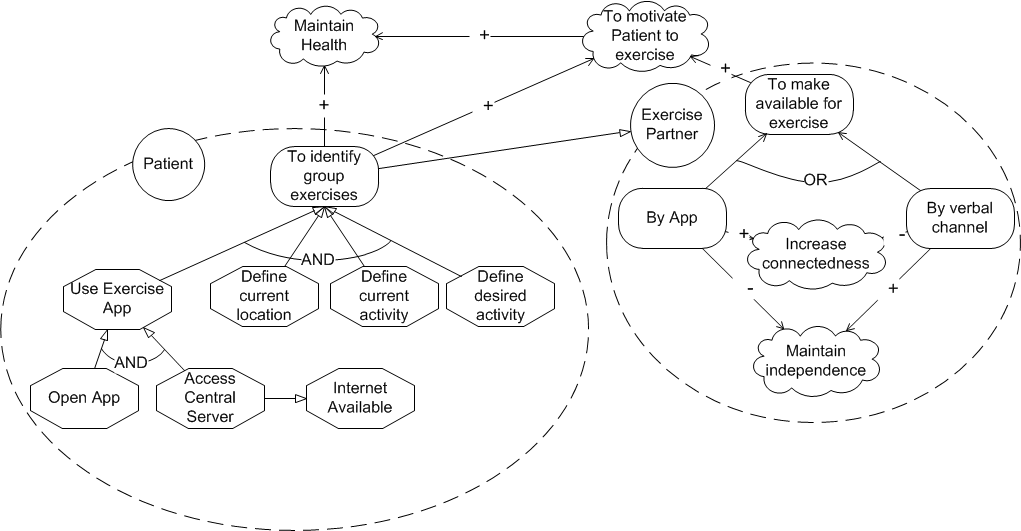
\includegraphics[scale=.51]{soc-r1-srgainey-as-is.png}}
\caption{Tropos As-Is model}
\label{fig:one}
\end{figure}

\begin{figure}
\centerline{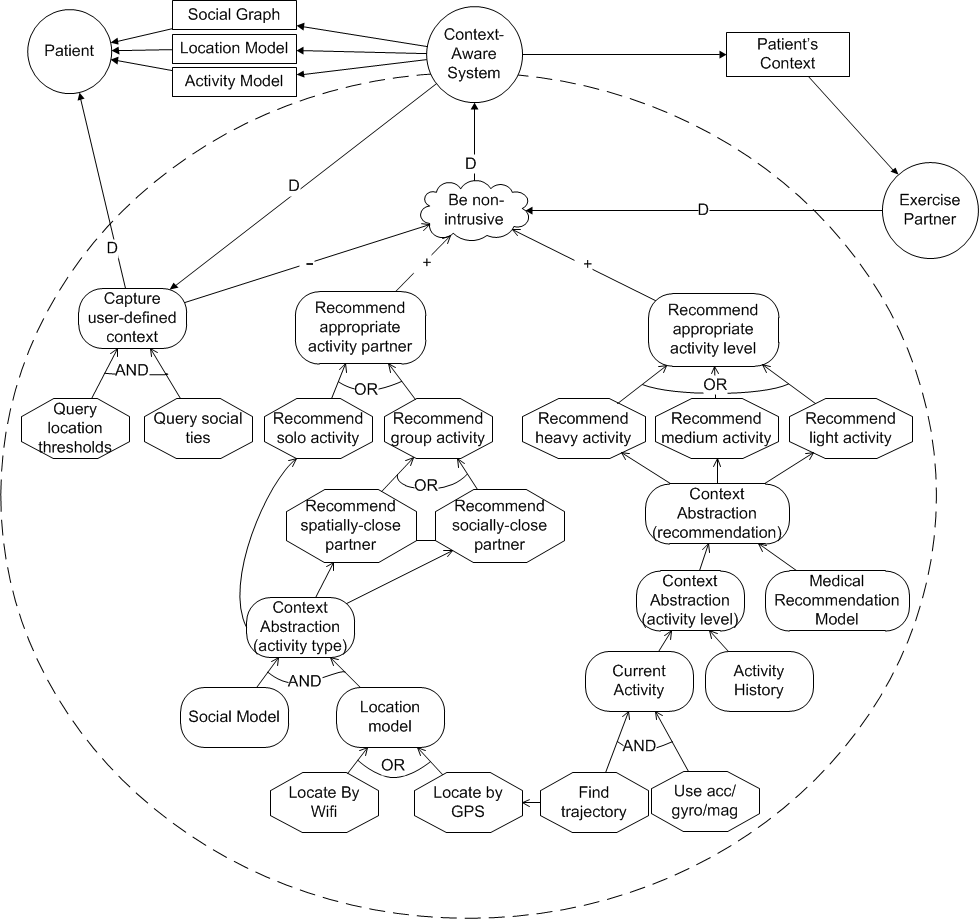
\includegraphics[scale=.51]{soc-r1-srgainey-to-be.png}}
\caption{Tropos To-Be model}
\label{fig:two}
\end{figure}

%\footnote{footnote here}

\begin{singlespace}
\begin{footnotesize}
\bibliography{soc-r1-srgainey}
\end{footnotesize}
\end{singlespace}

\end{document}